% Options for packages loaded elsewhere
\PassOptionsToPackage{unicode}{hyperref}
\PassOptionsToPackage{hyphens}{url}
%
\documentclass[
  9pt,
  ignorenonframetext,
  aspectratio=169]{beamer}
\usepackage{pgfpages}
\setbeamertemplate{caption}[numbered]
\setbeamertemplate{caption label separator}{: }
\setbeamercolor{caption name}{fg=normal text.fg}
\beamertemplatenavigationsymbolsempty
% Prevent slide breaks in the middle of a paragraph
\widowpenalties 1 10000
\raggedbottom
\setbeamertemplate{part page}{
  \centering
  \begin{beamercolorbox}[sep=16pt,center]{part title}
    \usebeamerfont{part title}\insertpart\par
  \end{beamercolorbox}
}
\setbeamertemplate{section page}{
  \centering
  \begin{beamercolorbox}[sep=12pt,center]{part title}
    \usebeamerfont{section title}\insertsection\par
  \end{beamercolorbox}
}
\setbeamertemplate{subsection page}{
  \centering
  \begin{beamercolorbox}[sep=8pt,center]{part title}
    \usebeamerfont{subsection title}\insertsubsection\par
  \end{beamercolorbox}
}
\AtBeginPart{
  \frame{\partpage}
}
\AtBeginSection{
  \ifbibliography
  \else
    \frame{\sectionpage}
  \fi
}
\AtBeginSubsection{
  \frame{\subsectionpage}
}
\usepackage{lmodern}
\usepackage{amssymb,amsmath}
\usepackage{ifxetex,ifluatex}
\ifnum 0\ifxetex 1\fi\ifluatex 1\fi=0 % if pdftex
  \usepackage[T1]{fontenc}
  \usepackage[utf8]{inputenc}
  \usepackage{textcomp} % provide euro and other symbols
\else % if luatex or xetex
  \usepackage{unicode-math}
  \defaultfontfeatures{Scale=MatchLowercase}
  \defaultfontfeatures[\rmfamily]{Ligatures=TeX,Scale=1}
\fi
\usetheme[]{Berkeley}
\usecolortheme{dove}
\usefonttheme{structurebold}
% Use upquote if available, for straight quotes in verbatim environments
\IfFileExists{upquote.sty}{\usepackage{upquote}}{}
\IfFileExists{microtype.sty}{% use microtype if available
  \usepackage[]{microtype}
  \UseMicrotypeSet[protrusion]{basicmath} % disable protrusion for tt fonts
}{}
\makeatletter
\@ifundefined{KOMAClassName}{% if non-KOMA class
  \IfFileExists{parskip.sty}{%
    \usepackage{parskip}
  }{% else
    \setlength{\parindent}{0pt}
    \setlength{\parskip}{6pt plus 2pt minus 1pt}}
}{% if KOMA class
  \KOMAoptions{parskip=half}}
\makeatother
\usepackage{xcolor}
\IfFileExists{xurl.sty}{\usepackage{xurl}}{} % add URL line breaks if available
\IfFileExists{bookmark.sty}{\usepackage{bookmark}}{\usepackage{hyperref}}
\hypersetup{
  pdftitle={Análise de variância e correlação},
  pdfauthor={Frederico Bertholini},
  hidelinks,
  pdfcreator={LaTeX via pandoc}}
\urlstyle{same} % disable monospaced font for URLs
\newif\ifbibliography
\usepackage{color}
\usepackage{fancyvrb}
\newcommand{\VerbBar}{|}
\newcommand{\VERB}{\Verb[commandchars=\\\{\}]}
\DefineVerbatimEnvironment{Highlighting}{Verbatim}{commandchars=\\\{\}}
% Add ',fontsize=\small' for more characters per line
\usepackage{framed}
\definecolor{shadecolor}{RGB}{248,248,248}
\newenvironment{Shaded}{\begin{snugshade}}{\end{snugshade}}
\newcommand{\AlertTok}[1]{\textcolor[rgb]{0.94,0.16,0.16}{#1}}
\newcommand{\AnnotationTok}[1]{\textcolor[rgb]{0.56,0.35,0.01}{\textbf{\textit{#1}}}}
\newcommand{\AttributeTok}[1]{\textcolor[rgb]{0.77,0.63,0.00}{#1}}
\newcommand{\BaseNTok}[1]{\textcolor[rgb]{0.00,0.00,0.81}{#1}}
\newcommand{\BuiltInTok}[1]{#1}
\newcommand{\CharTok}[1]{\textcolor[rgb]{0.31,0.60,0.02}{#1}}
\newcommand{\CommentTok}[1]{\textcolor[rgb]{0.56,0.35,0.01}{\textit{#1}}}
\newcommand{\CommentVarTok}[1]{\textcolor[rgb]{0.56,0.35,0.01}{\textbf{\textit{#1}}}}
\newcommand{\ConstantTok}[1]{\textcolor[rgb]{0.00,0.00,0.00}{#1}}
\newcommand{\ControlFlowTok}[1]{\textcolor[rgb]{0.13,0.29,0.53}{\textbf{#1}}}
\newcommand{\DataTypeTok}[1]{\textcolor[rgb]{0.13,0.29,0.53}{#1}}
\newcommand{\DecValTok}[1]{\textcolor[rgb]{0.00,0.00,0.81}{#1}}
\newcommand{\DocumentationTok}[1]{\textcolor[rgb]{0.56,0.35,0.01}{\textbf{\textit{#1}}}}
\newcommand{\ErrorTok}[1]{\textcolor[rgb]{0.64,0.00,0.00}{\textbf{#1}}}
\newcommand{\ExtensionTok}[1]{#1}
\newcommand{\FloatTok}[1]{\textcolor[rgb]{0.00,0.00,0.81}{#1}}
\newcommand{\FunctionTok}[1]{\textcolor[rgb]{0.00,0.00,0.00}{#1}}
\newcommand{\ImportTok}[1]{#1}
\newcommand{\InformationTok}[1]{\textcolor[rgb]{0.56,0.35,0.01}{\textbf{\textit{#1}}}}
\newcommand{\KeywordTok}[1]{\textcolor[rgb]{0.13,0.29,0.53}{\textbf{#1}}}
\newcommand{\NormalTok}[1]{#1}
\newcommand{\OperatorTok}[1]{\textcolor[rgb]{0.81,0.36,0.00}{\textbf{#1}}}
\newcommand{\OtherTok}[1]{\textcolor[rgb]{0.56,0.35,0.01}{#1}}
\newcommand{\PreprocessorTok}[1]{\textcolor[rgb]{0.56,0.35,0.01}{\textit{#1}}}
\newcommand{\RegionMarkerTok}[1]{#1}
\newcommand{\SpecialCharTok}[1]{\textcolor[rgb]{0.00,0.00,0.00}{#1}}
\newcommand{\SpecialStringTok}[1]{\textcolor[rgb]{0.31,0.60,0.02}{#1}}
\newcommand{\StringTok}[1]{\textcolor[rgb]{0.31,0.60,0.02}{#1}}
\newcommand{\VariableTok}[1]{\textcolor[rgb]{0.00,0.00,0.00}{#1}}
\newcommand{\VerbatimStringTok}[1]{\textcolor[rgb]{0.31,0.60,0.02}{#1}}
\newcommand{\WarningTok}[1]{\textcolor[rgb]{0.56,0.35,0.01}{\textbf{\textit{#1}}}}
\usepackage{graphicx}
\makeatletter
\def\maxwidth{\ifdim\Gin@nat@width>\linewidth\linewidth\else\Gin@nat@width\fi}
\def\maxheight{\ifdim\Gin@nat@height>\textheight\textheight\else\Gin@nat@height\fi}
\makeatother
% Scale images if necessary, so that they will not overflow the page
% margins by default, and it is still possible to overwrite the defaults
% using explicit options in \includegraphics[width, height, ...]{}
\setkeys{Gin}{width=\maxwidth,height=\maxheight,keepaspectratio}
% Set default figure placement to htbp
\makeatletter
\def\fps@figure{htbp}
\makeatother
\setlength{\emergencystretch}{3em} % prevent overfull lines
\providecommand{\tightlist}{%
  \setlength{\itemsep}{0pt}\setlength{\parskip}{0pt}}
\setcounter{secnumdepth}{5}

\title{Análise de variância e correlação}
\subtitle{Métodos Quantitativos Aplicados à Ciência Política}
\author{Frederico Bertholini}
\date{07.dez.2020}

\begin{document}
\frame{\titlepage}

\begin{frame}[allowframebreaks]
  \tableofcontents[hideallsubsections]
\end{frame}
\hypertarget{formalizando-hipuxf3teses}{%
\section{Formalizando Hipóteses}\label{formalizando-hipuxf3teses}}

\begin{frame}{Diferença entre médias (amostras não pareadas)}
\protect\hypertarget{diferenuxe7a-entre-muxe9dias-amostras-nuxe3o-pareadas}{}
\(H_0:\text{A média de notas de casados e solteiros é igual}\) ou
\(H_0:\mu_c-\mu_s=0\) ou \(H_0:\mu_c = \mu_s\)

\(H_1:\text{A média de notas de casados e solteiros é diferente}\) ou
\(H_1:\mu_c-\mu_s \neq 0\) ou \(H_1:\mu_c \neq \mu_s\)

Variável \textbf{dependente}: Notas

Variável \textbf{independente}: Situação conjugal

O que eu quero testar? Se a situação conjugal \emph{faz diferença} na
nota.

É \textbf{efeito}? Não! (Pearl, 2020) Inferência vs.~Causalidade
\end{frame}

\begin{frame}[fragile]{Como testar na prática? Distribuições:}
\protect\hypertarget{como-testar-na-pruxe1tica-distribuiuxe7uxf5es}{}
\begin{Shaded}
\begin{Highlighting}[]
\NormalTok{dfe }\OperatorTok{\%\textgreater{}\%}\StringTok{ }\KeywordTok{drop\_na}\NormalTok{(estcivil) }\OperatorTok{\%\textgreater{}\%}\StringTok{ }
\StringTok{  }\KeywordTok{ggplot}\NormalTok{(}\KeywordTok{aes}\NormalTok{(}\DataTypeTok{fill=}\NormalTok{estcivil,}\DataTypeTok{x=}\NormalTok{media,}\DataTypeTok{color=}\NormalTok{estcivil,}\DataTypeTok{group=}\NormalTok{estcivil)) }\OperatorTok{+}
\StringTok{  }\KeywordTok{geom\_density}\NormalTok{(}\DataTypeTok{color=}\OtherTok{NA}\NormalTok{,}\DataTypeTok{alpha=}\NormalTok{.}\DecValTok{65}\NormalTok{) }\OperatorTok{+}\StringTok{  }
\StringTok{  }\KeywordTok{geom\_vline}\NormalTok{(}\DataTypeTok{data=}\NormalTok{. }\OperatorTok{\%\textgreater{}\%}\StringTok{ }\KeywordTok{group\_by}\NormalTok{(estcivil) }\OperatorTok{\%\textgreater{}\%}\StringTok{ }\KeywordTok{summarise}\NormalTok{(}\DataTypeTok{media=}\KeywordTok{mean}\NormalTok{(media,}\DataTypeTok{na.rm =}\NormalTok{ T)),}
             \DataTypeTok{size=}\DecValTok{2}\NormalTok{,}\KeywordTok{aes}\NormalTok{(}\DataTypeTok{xintercept=}\NormalTok{media,}\DataTypeTok{color=}\NormalTok{estcivil)) }\OperatorTok{+}\StringTok{ }
\StringTok{  }\KeywordTok{guides}\NormalTok{(}\DataTypeTok{color=}\StringTok{"none"}\NormalTok{) }\OperatorTok{+}\StringTok{ }\NormalTok{theme\_ipsum\_mod}
\end{Highlighting}
\end{Shaded}

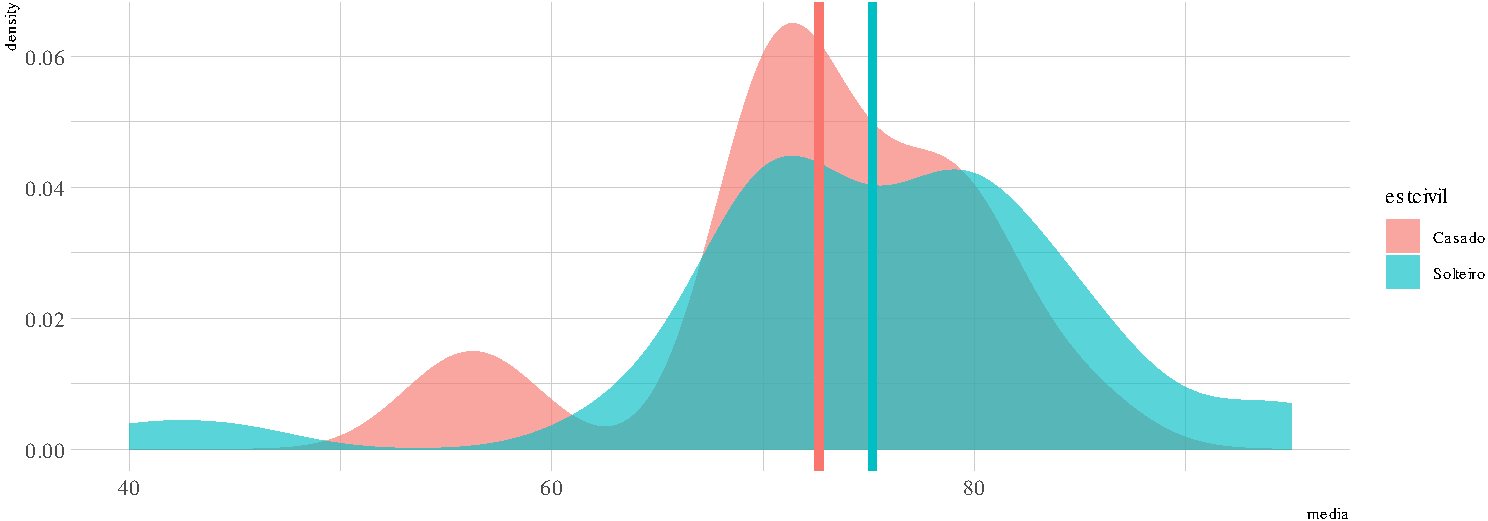
\includegraphics{aula_11_files/figure-beamer/unnamed-chunk-1-1.pdf}
\end{frame}

\begin{frame}[fragile]{Como testar na prática? Vamos construir
intervalos}
\protect\hypertarget{como-testar-na-pruxe1tica-vamos-construir-intervalos}{}
\begin{Shaded}
\begin{Highlighting}[]
\NormalTok{dfe }\OperatorTok{\%\textgreater{}\%}\StringTok{ }\KeywordTok{drop\_na}\NormalTok{(estcivil) }\OperatorTok{\%\textgreater{}\%}\StringTok{ }
\StringTok{  }\KeywordTok{ggplot}\NormalTok{(}\KeywordTok{aes}\NormalTok{(}\DataTypeTok{fill=}\NormalTok{estcivil,}\DataTypeTok{x=}\NormalTok{media,}\DataTypeTok{color=}\NormalTok{estcivil,}\DataTypeTok{y=}\NormalTok{estcivil)) }\OperatorTok{+}
\StringTok{  }\KeywordTok{stat\_summary}\NormalTok{(}\DataTypeTok{fun=}\NormalTok{mean, }\DataTypeTok{geom=}\StringTok{"point"}\NormalTok{) }\OperatorTok{+}\StringTok{ }
\StringTok{  }\KeywordTok{stat\_summary}\NormalTok{(}\DataTypeTok{fun.data=}\NormalTok{mean\_cl\_boot, }\DataTypeTok{geom=}\StringTok{"errorbar"}\NormalTok{, }\DataTypeTok{width=}\FloatTok{0.2}\NormalTok{) }\OperatorTok{+}
\StringTok{  }\KeywordTok{geom\_vline}\NormalTok{(}\DataTypeTok{data=}\NormalTok{. }\OperatorTok{\%\textgreater{}\%}\StringTok{ }\KeywordTok{group\_by}\NormalTok{(estcivil) }\OperatorTok{\%\textgreater{}\%}\StringTok{ }\KeywordTok{summarise}\NormalTok{(}\DataTypeTok{media=}\KeywordTok{mean}\NormalTok{(media,}\DataTypeTok{na.rm =}\NormalTok{ T)),}
             \DataTypeTok{size=}\DecValTok{2}\NormalTok{,}\KeywordTok{aes}\NormalTok{(}\DataTypeTok{xintercept=}\NormalTok{media,}\DataTypeTok{color=}\NormalTok{estcivil)) }\OperatorTok{+}\StringTok{ }
\StringTok{  }\NormalTok{theme\_ipsum\_mod }\OperatorTok{+}\KeywordTok{theme}\NormalTok{(}\DataTypeTok{legend.position =} \StringTok{"none"}\NormalTok{)}
\end{Highlighting}
\end{Shaded}

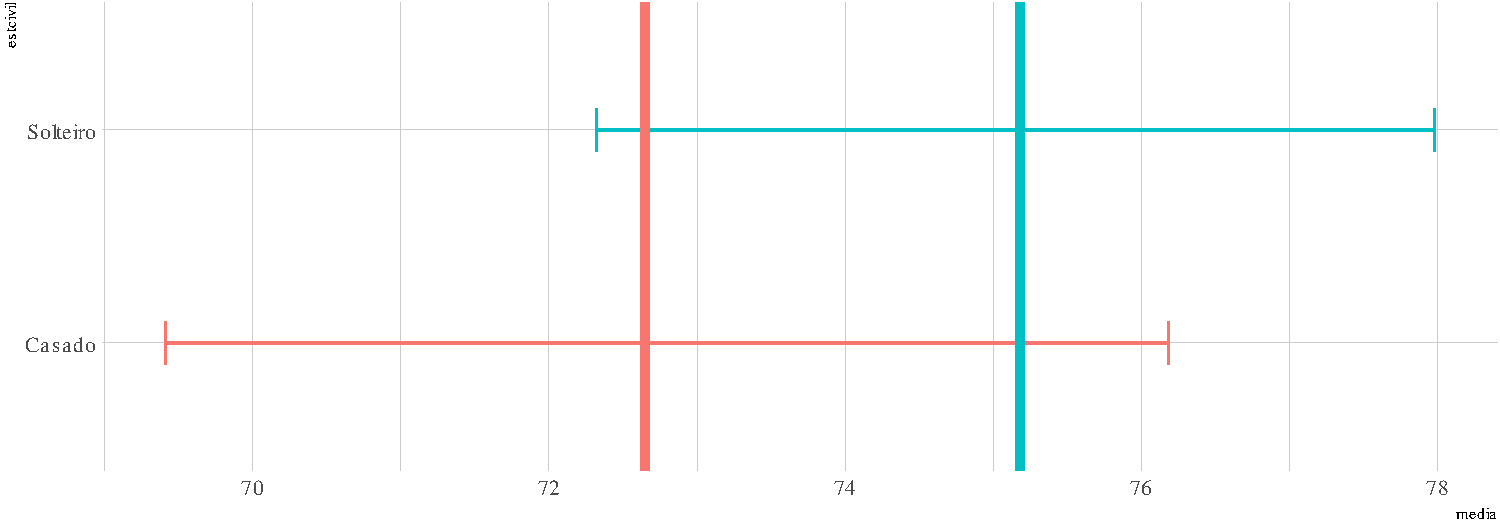
\includegraphics{aula_11_files/figure-beamer/unnamed-chunk-2-1.pdf}
\end{frame}

\begin{frame}[fragile]{Como testar na prática? Teste-t}
\protect\hypertarget{como-testar-na-pruxe1tica-teste-t}{}
\begin{Shaded}
\begin{Highlighting}[]
\NormalTok{t\_test\_results \textless{}{-}}\StringTok{ }\NormalTok{dfe }\OperatorTok{\%\textgreater{}\%}
\StringTok{  }\KeywordTok{t\_test}\NormalTok{(}\DataTypeTok{formula =}\NormalTok{ media }\OperatorTok{\textasciitilde{}}\StringTok{ }\NormalTok{estcivil,}
         \DataTypeTok{order =} \KeywordTok{c}\NormalTok{(}\StringTok{"Casado"}\NormalTok{, }\StringTok{"Solteiro"}\NormalTok{))}
\NormalTok{t\_test\_results}
\end{Highlighting}
\end{Shaded}

\begin{verbatim}
# A tibble: 1 x 6
  statistic  t_df p_value alternative lower_ci upper_ci
      <dbl> <dbl>   <dbl> <chr>          <dbl>    <dbl>
1     -1.03  40.4   0.311 two.sided      -7.52     2.46
\end{verbatim}
\end{frame}

\begin{frame}{Outro exercício}
\protect\hypertarget{outro-exercuxedcio}{}
\(H_0:\mu_\text{3joan} = \mu_\text{3joad}\)

\(H_1:\mu_\text{3joan} \neq \mu_\text{3joad}\)

Variável \textbf{dependente}: Notas

Variável \textbf{independente}: Turma (apenas 3joan e 3joad)
\end{frame}

\begin{frame}[fragile]{Intervalos}
\protect\hypertarget{intervalos}{}
\begin{Shaded}
\begin{Highlighting}[]
\NormalTok{dfe }\OperatorTok{\%\textgreater{}\%}\StringTok{ }\NormalTok{dplyr}\OperatorTok{::}\KeywordTok{filter}\NormalTok{(turma }\OperatorTok{\%in\%}\StringTok{ }\KeywordTok{c}\NormalTok{(}\StringTok{"3joan"}\NormalTok{,}\StringTok{"3joad"}\NormalTok{)) }\OperatorTok{\%\textgreater{}\%}\StringTok{ }
\StringTok{  }\KeywordTok{ggplot}\NormalTok{(}\KeywordTok{aes}\NormalTok{(}\DataTypeTok{fill=}\NormalTok{turma,}\DataTypeTok{x=}\NormalTok{media,}\DataTypeTok{color=}\NormalTok{turma,}\DataTypeTok{y=}\NormalTok{turma)) }\OperatorTok{+}
\StringTok{  }\KeywordTok{stat\_summary}\NormalTok{(}\DataTypeTok{fun=}\NormalTok{mean, }\DataTypeTok{geom=}\StringTok{"point"}\NormalTok{) }\OperatorTok{+}\StringTok{ }
\StringTok{  }\KeywordTok{stat\_summary}\NormalTok{(}\DataTypeTok{fun.data=}\NormalTok{mean\_cl\_boot, }\DataTypeTok{geom=}\StringTok{"errorbar"}\NormalTok{, }\DataTypeTok{width=}\FloatTok{0.2}\NormalTok{) }\OperatorTok{+}
\StringTok{  }\KeywordTok{geom\_vline}\NormalTok{(}\DataTypeTok{data=}\NormalTok{. }\OperatorTok{\%\textgreater{}\%}\StringTok{ }\KeywordTok{group\_by}\NormalTok{(turma) }\OperatorTok{\%\textgreater{}\%}\StringTok{ }\KeywordTok{summarise}\NormalTok{(}\DataTypeTok{media=}\KeywordTok{mean}\NormalTok{(media,}\DataTypeTok{na.rm =}\NormalTok{ T)),}
             \DataTypeTok{size=}\DecValTok{2}\NormalTok{,}\KeywordTok{aes}\NormalTok{(}\DataTypeTok{xintercept=}\NormalTok{media,}\DataTypeTok{color=}\NormalTok{turma)) }\OperatorTok{+}\StringTok{ }
\StringTok{  }\NormalTok{theme\_ipsum\_mod }\OperatorTok{+}\KeywordTok{theme}\NormalTok{(}\DataTypeTok{legend.position =} \StringTok{"none"}\NormalTok{)}
\end{Highlighting}
\end{Shaded}

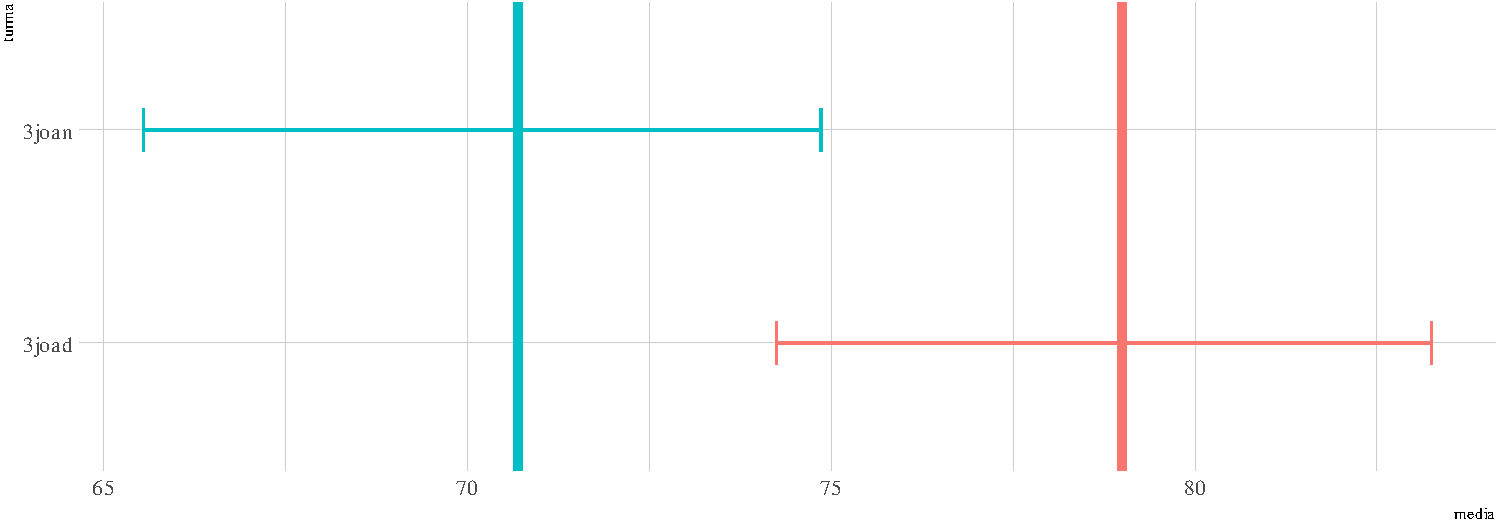
\includegraphics{aula_11_files/figure-beamer/unnamed-chunk-4-1.pdf}
\end{frame}

\begin{frame}[fragile]{Como testar na prática? Teste-t}
\protect\hypertarget{como-testar-na-pruxe1tica-teste-t-1}{}
\begin{Shaded}
\begin{Highlighting}[]
\NormalTok{t\_test\_results \textless{}{-}}\StringTok{ }\NormalTok{dfe }\OperatorTok{\%\textgreater{}\%}\StringTok{ }
\StringTok{  }\NormalTok{dplyr}\OperatorTok{::}\KeywordTok{filter}\NormalTok{(turma }\OperatorTok{\%in\%}\StringTok{ }\KeywordTok{c}\NormalTok{(}\StringTok{"3joan"}\NormalTok{,}\StringTok{"3joad"}\NormalTok{)) }\OperatorTok{\%\textgreater{}\%}\StringTok{ }
\StringTok{  }\KeywordTok{t\_test}\NormalTok{(}\DataTypeTok{formula =}\NormalTok{ media }\OperatorTok{\textasciitilde{}}\StringTok{ }\NormalTok{turma)}
\NormalTok{t\_test\_results}
\end{Highlighting}
\end{Shaded}

\begin{verbatim}
# A tibble: 1 x 6
  statistic  t_df p_value alternative lower_ci upper_ci
      <dbl> <dbl>   <dbl> <chr>          <dbl>    <dbl>
1      2.37  36.0  0.0232 two.sided       1.20     15.4
\end{verbatim}
\end{frame}

\begin{frame}[fragile]{Olhando no infer graficamente}
\protect\hypertarget{olhando-no-infer-graficamente}{}
\begin{Shaded}
\begin{Highlighting}[]
\CommentTok{\# calculate the observed statistic}
\NormalTok{media\_turmas \textless{}{-}}\StringTok{ }\NormalTok{dfe }\OperatorTok{\%\textgreater{}\%}\StringTok{ }
\StringTok{  }\NormalTok{dplyr}\OperatorTok{::}\KeywordTok{filter}\NormalTok{(turma }\OperatorTok{\%in\%}\StringTok{ }\KeywordTok{c}\NormalTok{(}\StringTok{"3joan"}\NormalTok{,}\StringTok{"3joad"}\NormalTok{)) }\OperatorTok{\%\textgreater{}\%}\StringTok{ }
\StringTok{  }\KeywordTok{specify}\NormalTok{(media }\OperatorTok{\textasciitilde{}}\StringTok{ }\NormalTok{turma) }\OperatorTok{\%\textgreater{}\%}
\StringTok{  }\KeywordTok{calculate}\NormalTok{(}\DataTypeTok{stat =} \StringTok{"t"}\NormalTok{, }\DataTypeTok{order =} \KeywordTok{c}\NormalTok{(}\StringTok{"3joan"}\NormalTok{,}\StringTok{"3joad"}\NormalTok{))}

\CommentTok{\# generate the null distribution with the theoretical t}
\NormalTok{distribuicao\_teorica \textless{}{-}}\StringTok{ }\NormalTok{dfe }\OperatorTok{\%\textgreater{}\%}\StringTok{ }
\StringTok{  }\NormalTok{dplyr}\OperatorTok{::}\KeywordTok{filter}\NormalTok{(turma }\OperatorTok{\%in\%}\StringTok{ }\KeywordTok{c}\NormalTok{(}\StringTok{"3joan"}\NormalTok{,}\StringTok{"3joad"}\NormalTok{)) }\OperatorTok{\%\textgreater{}\%}\StringTok{ }
\StringTok{  }\KeywordTok{specify}\NormalTok{(media }\OperatorTok{\textasciitilde{}}\StringTok{ }\NormalTok{turma) }\OperatorTok{\%\textgreater{}\%}
\StringTok{  }\KeywordTok{hypothesize}\NormalTok{(}\DataTypeTok{null =} \StringTok{"independence"}\NormalTok{) }\OperatorTok{\%\textgreater{}\%}
\StringTok{  }\KeywordTok{calculate}\NormalTok{(}\DataTypeTok{stat =} \StringTok{"t"}\NormalTok{, }\DataTypeTok{order =} \KeywordTok{c}\NormalTok{(}\StringTok{"3joan"}\NormalTok{,}\StringTok{"3joad"}\NormalTok{))}
\end{Highlighting}
\end{Shaded}
\end{frame}

\begin{frame}[fragile]{Visualizando}
\protect\hypertarget{visualizando}{}
\begin{Shaded}
\begin{Highlighting}[]
\CommentTok{\# visualize the randomization{-}based null distribution and test statistic!}
\NormalTok{distribuicao\_teorica }\OperatorTok{\%\textgreater{}\%}
\StringTok{  }\KeywordTok{visualize}\NormalTok{(}\DataTypeTok{method =} \StringTok{"theoretical"}\NormalTok{) }\OperatorTok{+}\StringTok{ }
\StringTok{  }\KeywordTok{shade\_p\_value}\NormalTok{(media\_turmas,}\DataTypeTok{direction =} \StringTok{"two{-}sided"}\NormalTok{) }\OperatorTok{+}\StringTok{ }
\StringTok{  }\KeywordTok{labs}\NormalTok{(}\DataTypeTok{title =} \StringTok{"Distribuição teórica"}\NormalTok{,}\DataTypeTok{x=}\StringTok{"Estatística t"}\NormalTok{,}\DataTypeTok{y=}\StringTok{"Densidade"}\NormalTok{)}
\end{Highlighting}
\end{Shaded}

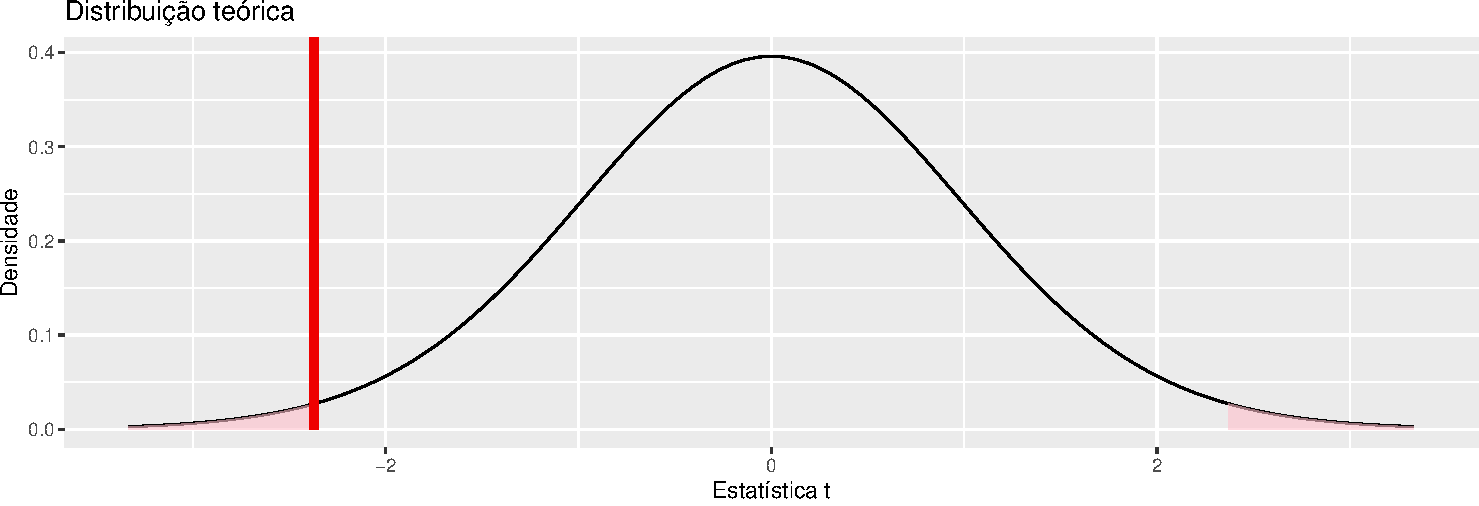
\includegraphics{aula_11_files/figure-beamer/unnamed-chunk-7-1.pdf}
\end{frame}

\begin{frame}[fragile]{Usando ggpubr}
\protect\hypertarget{usando-ggpubr}{}
\begin{Shaded}
\begin{Highlighting}[]
\KeywordTok{library}\NormalTok{(ggpubr)}
\NormalTok{dfe }\OperatorTok{\%\textgreater{}\%}\StringTok{ }\NormalTok{dplyr}\OperatorTok{::}\KeywordTok{filter}\NormalTok{(turma }\OperatorTok{\%in\%}\StringTok{ }\KeywordTok{c}\NormalTok{(}\StringTok{"3joan"}\NormalTok{,}\StringTok{"3joad"}\NormalTok{)) }\OperatorTok{\%\textgreater{}\%}\StringTok{ }
\StringTok{  }\KeywordTok{ggerrorplot}\NormalTok{(}\DataTypeTok{x =} \StringTok{"turma"}\NormalTok{, }\DataTypeTok{y =} \StringTok{"media"}\NormalTok{,}\DataTypeTok{color =} \StringTok{"turma"}\NormalTok{,}
              \DataTypeTok{position =} \KeywordTok{position\_dodge}\NormalTok{(}\FloatTok{0.5}\NormalTok{)) }\OperatorTok{+}
\StringTok{  }\KeywordTok{stat\_compare\_means}\NormalTok{(}\KeywordTok{aes}\NormalTok{(}\DataTypeTok{label =} \KeywordTok{paste0}\NormalTok{(..p.signif..,}\StringTok{" ou p = "}\NormalTok{, ..p.format..)),}
                     \DataTypeTok{method =} \StringTok{"t.test"}\NormalTok{) }\OperatorTok{+}\StringTok{ }\KeywordTok{theme}\NormalTok{(}\DataTypeTok{legend.position =} \StringTok{"right"}\NormalTok{)}
\end{Highlighting}
\end{Shaded}

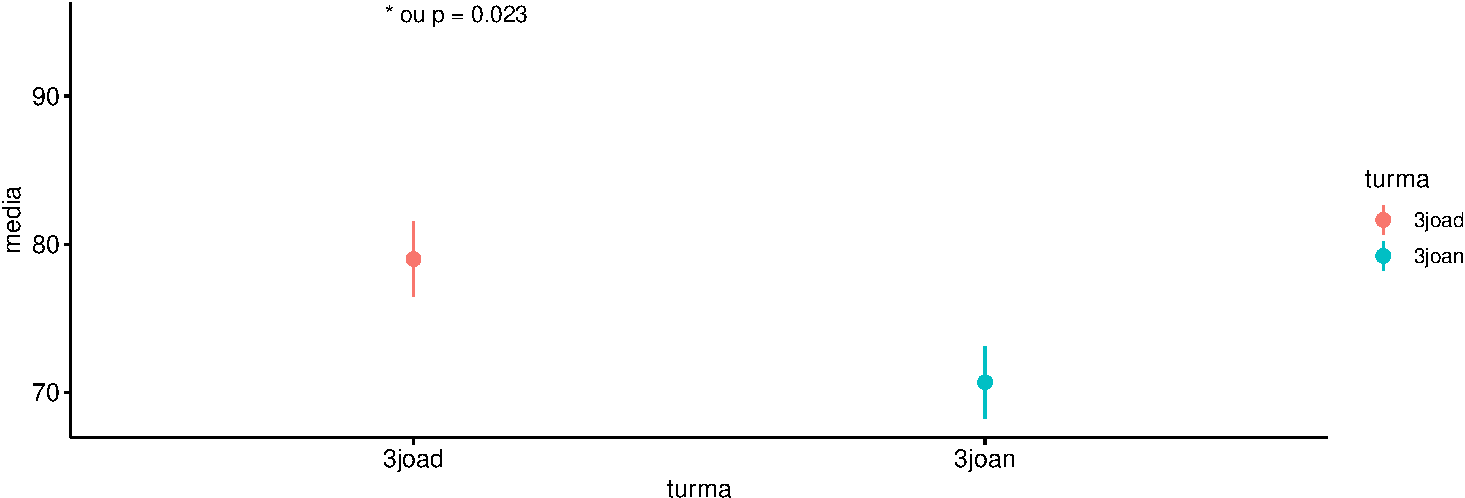
\includegraphics{aula_11_files/figure-beamer/unnamed-chunk-8-1.pdf}
\end{frame}

\begin{frame}{Tamanho do efeito}
\protect\hypertarget{tamanho-do-efeito}{}
\end{frame}

\begin{frame}{}
\protect\hypertarget{section}{}
\end{frame}

\hypertarget{testando-diferentes-hipuxf3teses}{%
\section{Testando diferentes
hipóteses}\label{testando-diferentes-hipuxf3teses}}

\begin{frame}{Por que ANOVA?}
\protect\hypertarget{por-que-anova}{}
\[
H_{0}: \mu_{1}=\mu_{2}=\cdots=\mu_{k}, \quad H_{A}: \mu_{i} \neq \mu_{j} \text{ para pelo menos um par } i \text{ e } j
\]
\end{frame}

\begin{frame}{O que é ANOVA?}
\protect\hypertarget{o-que-uxe9-anova}{}
\end{frame}

\begin{frame}{Na prática}
\protect\hypertarget{na-pruxe1tica}{}
\(H_0:\text{A média de notas das turmas é igual}\) ou
\(H_0:\mu_\text{3joad}=\mu_\text{3joan}=\mu_\text{5joan}\)

\(H_A:\text{A média de notas de pelo menos uma das turmas é diferente}\)
ou \(H_A:\mu_\text{3joad} \neq \mu_\text{3joan} \neq \mu_\text{5joan}\)

Variável dependente: Notas

Variável independente: Situação conjugal
\end{frame}

\hypertarget{medidas-de-associauxe7uxe3o}{%
\section{Medidas de associação}\label{medidas-de-associauxe7uxe3o}}

\hypertarget{modelo-linear-simples}{%
\section{Modelo Linear Simples}\label{modelo-linear-simples}}

\begin{frame}[fragile]{Modelo Linear Simples}
Nesta primeira aula, veremos um dos modelos mais básicos, mas também um
dos mais utilizados, de regressão: o modelo linear simples estimado por
mínimos quadrados ordinários (MQO).\footnote<.->{Para um explicação
  rápida de como esse método de estimação funciona,
  \href{https://fmeireles.shinyapps.io/modelagem_r/}{ver aqui}.} Entre
outros, aprenderamos a visualizar relações lineares bivariadas; a usar a
função básica para estimar modelos lineares, \texttt{lm}; e a obter
resultados detalhados de um modelo. Também usaremos alguns dados, que
estão na pasta de materiais desta aula.
\end{frame}

\begin{frame}[fragile]{Visualizando relações entre duas variáveis}
\protect\hypertarget{visualizando-relauxe7uxf5es-entre-duas-variuxe1veis}{}
Podemos usar gráficos para visualizar relações entre variáveis. Podemos,
por exemplo, criar duas variáveis contínuas, geradas aleatoriamente com
a função \texttt{rnorm}, e plotar sua relação com um gráfico de pontos.

\begin{Shaded}
\begin{Highlighting}[]
\KeywordTok{set.seed}\NormalTok{(}\DecValTok{123}\NormalTok{) }\CommentTok{\# Para replicar o conteudo da aula}

\NormalTok{x \textless{}{-}}\StringTok{ }\KeywordTok{rnorm}\NormalTok{(}\DecValTok{100}\NormalTok{)}
\NormalTok{y \textless{}{-}}\StringTok{ }\KeywordTok{rnorm}\NormalTok{(}\DecValTok{100}\NormalTok{)}

\KeywordTok{plot}\NormalTok{(y }\OperatorTok{\textasciitilde{}}\StringTok{ }\NormalTok{x)}
\end{Highlighting}
\end{Shaded}

É possível ver que as variáveis que criamos, \texttt{y} e \texttt{x},
não parecem ter relação. Na verdade, os pontos no gráficos estão
dispersos, o que dificulta detectar algum padrão.

Para investigarmos isso detidamente, usamos um modelo linear estimado
por mínimos quadrados ordinários (MQO). A função que estima esse tipo de
modelo chama-se \texttt{lm}, e ela está contida no \texttt{R-base}.
Portanto, não precisamos carregar nenhum pacote para usá-la, basta
executar o seguinte código:

\begin{Shaded}
\begin{Highlighting}[]
\KeywordTok{lm}\NormalTok{(y }\OperatorTok{\textasciitilde{}}\StringTok{ }\NormalTok{x)}
\end{Highlighting}
\end{Shaded}

A utilização da função \texttt{lm} é simples. Em primeiro lugar,
precisamos passar como argumento da função uma fórmula contendo a
especificação do nosso modelo. No exemplo, \texttt{y} é nossa variável
dependente e, assim, aparece do lado direito do operador
\texttt{\textasciitilde{}}. \texttt{x}, dessa forma, é nossa variável
independente, ou explicativa, ou, ainda, preditora.

Podemos salvar os resultados de um modelo em um objeto para facilitar a
sua manipulação.

\begin{Shaded}
\begin{Highlighting}[]
\NormalTok{meu\_modelo \textless{}{-}}\StringTok{ }\KeywordTok{lm}\NormalTok{(y }\OperatorTok{\textasciitilde{}}\StringTok{ }\NormalTok{x)}
\end{Highlighting}
\end{Shaded}

Uma das vantagens disso é que, agora, podemos usá-lo para traçar um reta
com valores preditos de \texttt{y} em relação a \texttt{x}, que resume a
relação entre ambas, no gráfico que criamos anteriormente. Para tanto,
usamos apenas a função \texttt{abline}.

\begin{Shaded}
\begin{Highlighting}[]
\KeywordTok{plot}\NormalTok{(y }\OperatorTok{\textasciitilde{}}\StringTok{ }\NormalTok{x)}
\KeywordTok{abline}\NormalTok{(meu\_modelo)}
\end{Highlighting}
\end{Shaded}

Realmente, não parece haver relação substantiva entre \texttt{y} e
\texttt{x}, como indica a melhor reta estimada via MQO.
\end{frame}

\begin{frame}[fragile]{Visualizando relações entre variáveis em um
banco}
\protect\hypertarget{visualizando-relauxe7uxf5es-entre-variuxe1veis-em-um-banco}{}
Daqui até o fim dessa aula, usaremos um banco de dados como exemplo para
praticarmos o básico de construção de modelos bivariados. Esse arquivo,
com algumas variáveis selecionadas do Atlas do Desenvolvimento Humano
para municípios no ano de 2010
(\url{http://atlasbrasil.org.br/2013/pt/download/}), chama-se
\texttt{atlas\_condensado.csv}, e está nos materiais complementares
dessa aula. Como ele está no formato \texttt{.csv}, podemos carregá-lo
com a função \texttt{read\_csv} do pacote \texttt{readr}, salvando o
banco num objeto \texttt{atlas}.

\begin{Shaded}
\begin{Highlighting}[]
\KeywordTok{library}\NormalTok{(readr)}
\NormalTok{atlas \textless{}{-}}\StringTok{ }\KeywordTok{read\_csv}\NormalTok{(}\StringTok{"atlas\_condensado.csv"}\NormalTok{)}
\end{Highlighting}
\end{Shaded}

A função \texttt{read\_csv} já indica o nome e a classe de cada variável
no objeto \texttt{atlas}, onde salvamos os dados. Usando \texttt{names}
e \texttt{head}, é possível ver mais detalhadamente esse
\texttt{data.frame}.

\begin{Shaded}
\begin{Highlighting}[]
\KeywordTok{names}\NormalTok{(atlas)}
\KeywordTok{head}\NormalTok{(atlas)}
\end{Highlighting}
\end{Shaded}

Em particular, vamos trabalhar com duas dessas variáveis: a
\texttt{t\_agua}, que indica a percentagem de domicílios com água
encanada, e a \texttt{mort1}, que indica o número de crianças que não
sobreviveram ao primeiro ano de idade em cada 1000 crianças nascidas no
município. Nosso objetivo será investigar se existe relação entre
disponibilidade de água encanada (nossa variável independente) e
mortalidade infantil (nossa variável dependente) usando um modelo linear
por MQO. Como essas variáveis estão dentro de um banco de dados, existe
um modo mais fácil de visualizar a relação entre elas usando o pacote
\texttt{ggplot2}. Especificamente, esse pacote contém um \texttt{geom}
chamado \texttt{geom\_smooth} que serve para plotar uma curva trançando
a relação entre duas (ou mais, como veremos adiante) variáveis. Criamos
esse gráfico com o seguinte código:

\begin{Shaded}
\begin{Highlighting}[]
\KeywordTok{ggplot}\NormalTok{(atlas, }\KeywordTok{aes}\NormalTok{(}\DataTypeTok{x =}\NormalTok{ t\_lixo, }\DataTypeTok{y =}\NormalTok{ mort1)) }\OperatorTok{+}\StringTok{ }
\StringTok{  }\KeywordTok{geom\_point}\NormalTok{() }\OperatorTok{+}\StringTok{ }\CommentTok{\# Adiciona os pontos}
\StringTok{  }\KeywordTok{geom\_smooth}\NormalTok{(}\DataTypeTok{method =} \StringTok{"lm"}\NormalTok{) }\CommentTok{\# Adiciona a curva, estimada por um modelo linear}
\end{Highlighting}
\end{Shaded}

Como se depreende do código acima, só precisamos especificar um método
na função \texttt{geom\_smooth} que, no caso, é \texttt{"lm"}, de
\emph{linear model}. Mais importante, nesse caso parece haver uma clara
associação negativa entre a disponibilidade domiciliar de água e
mortalidade infantil: quanto maior a disponibilidade, menor a
mortalidade.
\end{frame}

\begin{frame}[fragile]{Estimativas}
\protect\hypertarget{estimativas}{}
Para examinarmos formalmente a relação entre \texttt{t\_agua} e
\texttt{mort1}, vamos recorrer novamente à função \texttt{lm}. Como
temos um \texttt{data.frame} agora, e não mais dois vetores em objetos
diferentes, usaremos um argumento da função \texttt{lm} para passar as
variáveis do banco para ela. O argumento chama-se \texttt{data\ =}, e
precisamos apenas passar a ele o nome do \texttt{data.frame} que contém
nossas variáveis.

\begin{Shaded}
\begin{Highlighting}[]
\NormalTok{meu\_modelo \textless{}{-}}\StringTok{ }\KeywordTok{lm}\NormalTok{(mort1 }\OperatorTok{\textasciitilde{}}\StringTok{ }\NormalTok{t\_agua, }\DataTypeTok{data =}\NormalTok{ atlas)}
\end{Highlighting}
\end{Shaded}

Note que podemos estimar o mesmo modelo sem usar o argumento
\texttt{data}, mas precisaremos usar em seu lugar indexadores (o que é
mais trabalhoso e não recomendado):

\begin{Shaded}
\begin{Highlighting}[]
\KeywordTok{lm}\NormalTok{(atlas}\OperatorTok{$}\NormalTok{mort1 }\OperatorTok{\textasciitilde{}}\StringTok{ }\NormalTok{atlas}\OperatorTok{$}\NormalTok{t\_agua)}
\end{Highlighting}
\end{Shaded}

Para exibir de forma condensada os resultados do nosso modelo salvo em
\texttt{meu\_modelo}, basta digitar o nome do objeto no console:

\begin{Shaded}
\begin{Highlighting}[]
\NormalTok{meu\_modelo}
\end{Highlighting}
\end{Shaded}

Os dois modos produzem o mesmo resultado, ainda que o segundo seja o
mais adequado. Mas, afinal, o que significa esse output da função
\texttt{lm}. Podemos resumi-lo em duas partes:

\begin{itemize}
\item
  \begin{enumerate}
  \tightlist
  \item
    Abaixo de \texttt{Call:}, a função \texttt{lm} apenas exibe a
    chamada que usamos para rodar nosso modelo, incluindo aqui a fórmula
    usada;
  \end{enumerate}
\item
  \begin{enumerate}
  \setcounter{enumi}{1}
  \tightlist
  \item
    O mais importante, contudo, segue abaixo de \texttt{Coefficients:},
    indicando a estimativa dos parâmetros, ou coeficientes, do efeito da
    variável independente, \texttt{t\_agua}, sobre a variável
    dependente, \texttt{mort1}, além de um intercepto (ou constante),
    que indica o valor de esperado de mortalidade infantil num município
    hipotético onde a disponibilidade de água nos domicílios é zero.
  \end{enumerate}
\end{itemize}

Com isso, podemos concluir rapidamente que a associação entre
\texttt{t\_agua} e \texttt{mort1} é negativa, uma vez que um aumento de
1\% da variável \texttt{t\_agua} prediz um decréscimo em \texttt{mort1}.
Além disso, quando o valor de \texttt{t\_agua} é igual a zero, nosso
modelo prediz que o valor de \texttt{mort1} será igual ao da estimativa
do intercepto. Obviamente, isso condiz o gráfico que fizemos
anteriormente.
\end{frame}

\begin{frame}[fragile]{Inferência}
\protect\hypertarget{inferuxeancia}{}
No mais das vezes, apenas avaliar um modelo pelos seus coeficientes não
é suficiente. Usando nosso modelo estimado, podemos facilmente dar um
passo adiante e fazer inferências a partir deles, considerando a
incerteza na estimação dos nossos parâmetros.

Para tanto, o \texttt{R} dispõe de uma função, que é carregada por
padrão a partir do pacote \texttt{stats}, chamada \texttt{confint}. Com
ela, é possível calcular um intervalo de confiança de 95\% (ou qualquer
outro valor) para os coeficientes de nosso modelo.

\begin{Shaded}
\begin{Highlighting}[]
\KeywordTok{confint}\NormalTok{(meu\_modelo, }\DataTypeTok{level =} \FloatTok{0.95}\NormalTok{)}
\end{Highlighting}
\end{Shaded}

A função retorna os intervalos mínimo e máximo de cada estimativa, o que
pode ser usado para fazer afirmações do tipo de que, com 95\% de
probabilidade, nossa estimativa do efeito de \texttt{t\_gua} sobre
\texttt{mort1} está situada no intervalo indicado por \texttt{2.5\ \%} e
\texttt{97.5\ \%}.

Para alterar a cobertura do intervalo de confiança, basta modificar o
valor passado ao argumento \texttt{level} da função (0.95 equivale a um
intervalo de 95\%):

\begin{Shaded}
\begin{Highlighting}[]
\KeywordTok{confint}\NormalTok{(meu\_modelo, }\DataTypeTok{level =} \FloatTok{0.90}\NormalTok{)}
\end{Highlighting}
\end{Shaded}
\end{frame}

\begin{frame}[fragile]{Obtendo resultados detalhados}
\protect\hypertarget{obtendo-resultados-detalhados}{}
Ainda que exibir os resultados da forma como fizemos seja útil para uma
inspeção rápida, existem outras informações úteis que precisamos acessar
para avaliarmos um modelo. Para obtê-las, usamos a função
\texttt{summary}, que já vimos anteriormente.

\begin{Shaded}
\begin{Highlighting}[]
\KeywordTok{summary}\NormalTok{(meu\_modelo)}
\end{Highlighting}
\end{Shaded}

Afora a linha iniciada por \texttt{Call:}, que já vimos, essa função
retorna uma série de novas informações. Vamos focar especialmente em
duas:

\begin{itemize}
\item
  \begin{enumerate}
  \tightlist
  \item
    \texttt{Coefficients:} reporta informações sobre as estimativas e
    inferências de nosso modelo, incluindo aqui a estimativa do efeito
    de nossas variáveis independentes e intercepto (abaixo de
    \texttt{Estimate}); o erro-padrão (\texttt{Std.\ Error}) de cada
    estimativa, que indica a incerteza envolvida nelas (e é usada no
    cálculo de intervalos de confiança); T-valor, \texttt{t\ value}, uma
    métrica normalmente usada para calcular P-valores em modelos de
    regressão (i.e., que é igual à estimativa divido pelo erro-padrão);
    e, finalmente, P-valor,
    \texttt{Pr(\textgreater{}\textbar{}t\textbar{})}, a famosa
    estatística usada para testar se o efeito indicado por cada
    estimativa é (P-valor \textgreater{} 0.05) ou não (P-valor
    \textless{} 0.05) fruto de variação aleatória.\footnote<.->{A título
      de curiosidade, o P-valor é calculado com base na estatística T de
      cada variável e outra informação que cobriremos a seguir, os graus
      de liberdade do modelo.};
  \end{enumerate}
\item
  \begin{enumerate}
  \setcounter{enumi}{1}
  \tightlist
  \item
    \texttt{Multiple\ R-squared:} e \texttt{Adjusted\ R-squared:} são
    métricas simples que indicam a quantia de variação explicada pelo
    nosso modelo, onde 1 indica que toda a variação é explicada (e,
    logo, nossas variáveis predizem perfeitamente os valores de Y);
  \end{enumerate}
\end{itemize}
\end{frame}

\begin{frame}[fragile]{Acessando informações de um objeto lm}
\protect\hypertarget{acessando-informauxe7uxf5es-de-um-objeto-lm}{}
Assim como outras informações no \texttt{R}, nosso modelo salvo no
objeto \texttt{meu\_modelo} contém diversas informações dentro dele. Por
exemplo, podemos extrair um vetor com nossas estimativas usando:

\begin{Shaded}
\begin{Highlighting}[]
\NormalTok{meu\_modelo}\OperatorTok{$}\NormalTok{coefficients}
\end{Highlighting}
\end{Shaded}

Essa e outras informações salvas dentro do objeto podem ser vistas com
\texttt{names}:

\begin{Shaded}
\begin{Highlighting}[]
\KeywordTok{names}\NormalTok{(meu\_modelo)}
\end{Highlighting}
\end{Shaded}

Também é possível salvar o \emph{output} da função \texttt{summary} para
fazer a mesma coisa.

\begin{Shaded}
\begin{Highlighting}[]
\NormalTok{resumo \textless{}{-}}\StringTok{ }\KeywordTok{summary}\NormalTok{(meu\_modelo)}
\end{Highlighting}
\end{Shaded}

Feito isso, temos à disposição todas as estatísticas reportadas pela
função \texttt{summary} dentro de um mesmo objeto, o que pode ser usado,
por exemplo, para extrair rapidamente apenas o R-quadrado de nosso
modelo, como abaixo.

\begin{Shaded}
\begin{Highlighting}[]
\NormalTok{resumo}\OperatorTok{$}\NormalTok{r.squared}
\end{Highlighting}
\end{Shaded}

Isso será bastante útil em algumas situações que veremos adiante. Por
enquanto, tente explorar as informações contidas dentro dos objetos
\texttt{resumo} e \texttt{meu\_modelo} e tente identificar o que
indicam.
\end{frame}

\begin{frame}[fragile]{Exercícios II}
\protect\hypertarget{exercuxedcios-ii}{}
\begin{itemize}
\item
  \begin{enumerate}
  [1)]
  \tightlist
  \item
    A base \texttt{atlas}, que carregamos anteriormente, contém outras
    duas variáveis que podem ter relação com a taxa de mortalidade
    infantial até um 1 ano por 1000 crianças nascidas. São elas:
    \texttt{t\_lixo}, que indica a \% de domicílios no município com
    coleta de lixo; e \texttt{t\_luz}, que indica a \% de domicílios com
    energia elétrica. Qual sua expectativa do efeito dessas variáveis
    sobre \texttt{mort1}?
  \end{enumerate}
\item
  \begin{enumerate}
  [1)]
  \setcounter{enumi}{1}
  \tightlist
  \item
    Faça dois gráficos de \emph{scatterplot}, um para investigar a
    relação entre \texttt{mort1} e \texttt{t\_luz} e, o outro, para
    investigar a relação entre \texttt{mort1} e \texttt{t\_lixo};
  \end{enumerate}
\item
  \begin{enumerate}
  [1)]
  \setcounter{enumi}{2}
  \tightlist
  \item
    Estime e salve dois modelos lineares simples para examinar a relação
    entre \texttt{mort1} e \texttt{t\_luz} e entre \texttt{mort1} e
    \texttt{t\_lixo}. Lembre-se: \texttt{mort1} é nossa variável
    dependente;
  \end{enumerate}
\item
  \begin{enumerate}
  [1)]
  \setcounter{enumi}{3}
  \tightlist
  \item
    Usando \texttt{summary}, interprete os resultados desses dois
    modelos. Os resultados condizem com a sua expectativa prévia?
  \end{enumerate}
\item
  \begin{enumerate}
  [1)]
  \setcounter{enumi}{4}
  \tightlist
  \item
    Com os mesmos modelos estimados anteriormente, faça inferência a
    partir do efeito de \texttt{t\_luz} e \texttt{t\_lixo} sobre
    \texttt{mort1}. Quais são os intervalos máximos e mínimos,
    considerando 95\% de probabilidade, dos efeitos dessas duas
    variáveis?
  \end{enumerate}
\end{itemize}
\end{frame}

\hypertarget{aula2}{%
\section{Modelos Lineares Multivariados}\label{aula2}}

\begin{frame}{Modelos Lineares Multivariados}
Embora examinar a relação entre duas variáveis, como vimos na Aula
@ref(aula1), seja útil em algumas ocasiões, modelos lineares também
servem para examinar o efeito de múltiplas variáveis independentes
simultaneamente. Nessa aula, vamos ver como estimar modelos como estes.
Após isso, veremos como rodar e interpretar de forma simples modelos
lineares multivariados e, também, modelos com transformações de
variáveis independentes -- o que é útil em alguns casos, como quando
examinamos relações quadráticas ou quando desejamos interpretar
coeficientes de forma percentual.
\end{frame}

\begin{frame}[fragile]{Modelo linear com dois preditores}
\protect\hypertarget{modelo-linear-com-dois-preditores}{}
No exemplo da Aula @ref(aula1), examinamos o efeito da variávei X sobre
Y em todos os municípios brasileiros. Como vimos, essa relação é
positiva e, além disso, é possível inferir isso a partir dos dados, dado
os intervalos de confiança da estimativa do efeito predito de X sobre Y.

Na mesma base de dados, também temos outra variável que possivelmente
tem efeito sobre Y. Essa variável chama-se \texttt{X}, e indica
quanto\ldots{}

Vamos carregar nosso banco de dados usando o pacote \texttt{readr}.

\begin{Shaded}
\begin{Highlighting}[]
\KeywordTok{library}\NormalTok{(readr)}
\NormalTok{x \textless{}{-}}\StringTok{ }\KeywordTok{read\_delim}\NormalTok{(}\StringTok{"afe.txt"}\NormalTok{, }\DataTypeTok{delim =} \StringTok{";"}\NormalTok{)}
\end{Highlighting}
\end{Shaded}

Para termos uma ideia sobre a distribuição da variável X, podemos usar o
indexador \texttt{\$} para acessá-la conjuntamente com a função
\texttt{summary} para gerar algumas estatísticas descritivas.

\begin{Shaded}
\begin{Highlighting}[]
\KeywordTok{summary}\NormalTok{(x}\OperatorTok{$}\NormalTok{variavel)}
\end{Highlighting}
\end{Shaded}

Sempre é uma boa ideia examinar graficamente a relação entre variáveis
e, nesse caso, podemos fazer isso usando o pacote \texttt{ggplot2} para
plotar a relação entre X e Y.

\begin{Shaded}
\begin{Highlighting}[]
\KeywordTok{library}\NormalTok{(ggplot2)}

\KeywordTok{ggplot}\NormalTok{(banco, }\KeywordTok{aes}\NormalTok{(}\DataTypeTok{x =}\NormalTok{ x, }\DataTypeTok{y =}\NormalTok{ y)) }\OperatorTok{+}\StringTok{ }
\StringTok{  }\KeywordTok{geom\_point}\NormalTok{() }\OperatorTok{+}\StringTok{ }
\StringTok{  }\KeywordTok{geom\_smooth}\NormalTok{(}\DataTypeTok{method =} \StringTok{"lm"}\NormalTok{) }
\end{Highlighting}
\end{Shaded}

O problema: essa relação não leva em conta o efeito de X. Talvez
municípios que tenham valores\ldots{} em X tenham \ldots{} em X2.
Modelos lineares nos permitem contornar esse tipo de problema. Para
isso, precisamos apenas estimar um modelo que inclua as duas variáveis,
X e X2, como preditores simultaneamente. O truque para fazer isso é
fácil: basta apenas usar um \texttt{+} para adicionar mais variáveis.

\begin{Shaded}
\begin{Highlighting}[]
\NormalTok{meu\_modelo2 \textless{}{-}}\StringTok{ }\KeywordTok{lm}\NormalTok{(y }\OperatorTok{\textasciitilde{}}\StringTok{ }\NormalTok{x }\OperatorTok{+}\StringTok{ }\NormalTok{x2, }\DataTypeTok{data =}\NormalTok{ banco)}
\end{Highlighting}
\end{Shaded}
\end{frame}

\begin{frame}[fragile]{Modelos com múltiplos preditores}
\protect\hypertarget{modelos-com-muxfaltiplos-preditores}{}
Usando a mesma sintaxe que vimos acima, podemos facilmente incluir mais
variáveis a um modelo linear. Vamos incluir uma variável adicional ao
nosso modelo, chamada X, que indica\ldots{}

\begin{Shaded}
\begin{Highlighting}[]
\NormalTok{meu\_modelo2 \textless{}{-}}\StringTok{ }\KeywordTok{lm}\NormalTok{(y }\OperatorTok{\textasciitilde{}}\StringTok{ }\NormalTok{x }\OperatorTok{+}\StringTok{ }\NormalTok{x2, }\DataTypeTok{data =}\NormalTok{ banco)}
\end{Highlighting}
\end{Shaded}

Aqui também, interpretar os resultados é algo simples.
\end{frame}

\begin{frame}[fragile]{Obtendo resultados simplificados}
\protect\hypertarget{obtendo-resultados-simplificados}{}
Algo que dificulta interpretar modelos multivariados de forma rápida é a
quantidade de informações reportada pela função \texttt{summary}.
Felizmente, existe uma alternativa a ela em um pacote chamado
\texttt{arm}: a função \texttt{display}. Em vez de reportar uma série de
estatísticas e informações nem sempre úteis, essa função simplifica os
resultados de uma regressão, reportando apenas estimativas, erros-padrão
e informações como número de observações e parâmetros estimados. Como
veremos adiante, \texttt{arm} também oferece algumas funções que
simplificam enormemente nossa tarefa de estimar e analisar modelos de
regressão.

Como esse pacote não vem por padrão no \texttt{R}, precisamos intalá-lo
usando \texttt{install.packages}.

\begin{Shaded}
\begin{Highlighting}[]
\KeywordTok{install.packages}\NormalTok{(arm)}
\end{Highlighting}
\end{Shaded}

Feito isso, podemos carregar o pacote e usá-lo para reportar os
resultados do nosso modelo linear multivariado salvo no objeto
\texttt{modelo\_multi}.

\begin{Shaded}
\begin{Highlighting}[]
\KeywordTok{library}\NormalTok{(arm)}

\KeywordTok{display}\NormalTok{(modelo\_multi)}
\end{Highlighting}
\end{Shaded}
\end{frame}

\begin{frame}[fragile]{Interpretando resultados com gráficos}
\protect\hypertarget{interpretando-resultados-com-gruxe1ficos}{}
\texttt{arm} ainda oferece um jeito mais fácil de visualizar resultados
de modelos multivariados. Usando a função \texttt{coefplot}, ele plota
as estimativas de um modelo, já incluindo intervalos de confiança de
95\% e 90\%. Para usá-la, basta passar o objeto com o modelo salvo para
a função.

\begin{Shaded}
\begin{Highlighting}[]
\KeywordTok{coefplot}\NormalTok{(modelo\_multi)}
\end{Highlighting}
\end{Shaded}

Além de simples, o resultado gráfico
\end{frame}

\begin{frame}{Centrando preditores}
\protect\hypertarget{centrando-preditores}{}
\end{frame}

\begin{frame}{Tranformando preditores}
\protect\hypertarget{tranformando-preditores}{}
\end{frame}

\begin{frame}{Relações quadráticas e outras}
\protect\hypertarget{relauxe7uxf5es-quadruxe1ticas-e-outras}{}
\end{frame}

\begin{frame}{Exercícios}
\protect\hypertarget{exercuxedcios}{}
\end{frame}

\end{document}
